\documentclass{article}[18pt]
\usepackage{../../../../../format}
\lhead{CT - Graphs}


\begin{document}
\begin{center}
\underline{\huge Graph colouring II}
\end{center}
\section{Graph Colouring}
A proper colouring of a graph with k colours:
\begin{itemize}
\item A colouring of the vertices, such that any two adjacent vertices have different colours
\end{itemize}
The graph colouring problem:
\begin{itemize}
\item Find the smallest number k such that the graph has a proper k colouring
\end{itemize}
A brute force algorithm for 3 colouring:
\begin{itemize}
\item exhaustively enumerate all possible 3-colourings
\item For each colouring, check whether all vertex pairs have different colours
\item correct answer is always guaranteed
\item Exponential time needed ($3^n$ iterations)
\end{itemize}
Sometimes we just want "some" proper colouring:
\begin{itemize}
\item not necessarily with the smallest number of colours
\item but we want it quickly
\end{itemize}
Then: a greedy algorithm
\section{A "greedy" algorithm}
\begin{itemize}
\item Assign labels to the vertices $v_1,v_2,v_3,v_4,...,v_n$ such that\\
$v_2$ is adjacent to $v_1$\\
$v_3$ is adjacent to one of $\{v_1,v_2\}$\\
$v_4$ is adjacent to one of $\{v_1,v_2,v_3\}$\\
...\\
$v_n$ is adjacent to one of $\{v_1,v_2,v_3,...,v_{n-1}\}$
\item Visit the vertices sequentially
\item Assign to each vertex the "smallest" colour that is not being used by its neighbours so far
\end{itemize}
\begin{center}
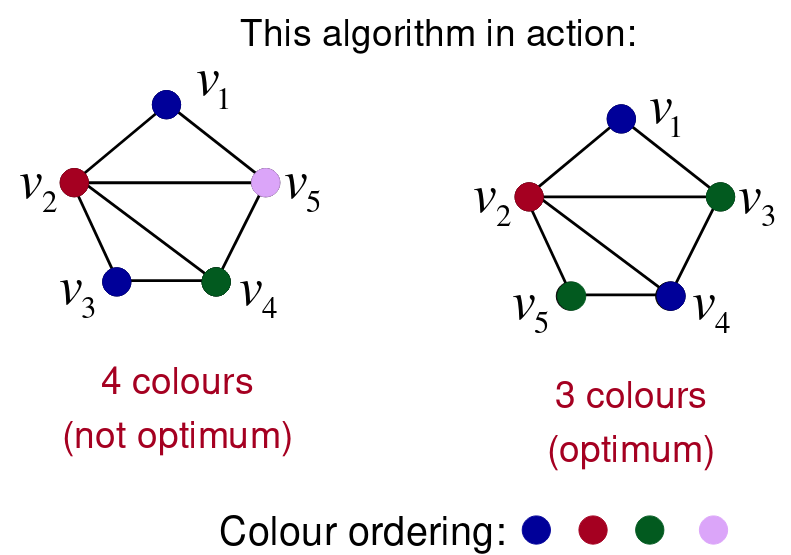
\includegraphics[scale=0.7]{greedy}
\end{center}
\begin{itemize}
\item This greedy algorithm:
\begin{itemize}
\item finishes quickly (polynomial number of iterations)
\item Makes at every step a decision that "looks the best for now"
\item but the final output may not be the best possible
\end{itemize}
\item The choice of vertex ordering:
\begin{itemize}
\item determines the quality of the solution (i.e. number of colours)
\end{itemize}
\item It is hard (NP-complete) to compute the best possible vertex ordering
\end{itemize}
\section{Which algorithm to choose}
\begin{tabular}{|c|c|c|}
\hline 
 & brute-force algorithm & greedy algorithm \\ 
\hline 
+ & computes always the optimum & finishes quickly (polynomial time) \\ 
\hline 
- & finishes very slowly (exponential time) & not always the optimum solution \\ 
\hline 
\end{tabular} \\
Two measures of algorithmic performance:
\begin{itemize}
\item quality of the solution (how far from the optimum)
\item time needed
\end{itemize}
\section{A "greedy" algorithm}
\begin{itemize}
	\item Ok, it is hard to find the optimum in general
	\item What is I just look for specific small values of k?
	\item For k=1
	\begin{itemize}
		\item only the trivial graph (one vertex) can be coloured with only one colour
	\end{itemize}
	\item For k=2 bipartite graphs
\end{itemize}
\section{Bipartite graph}
\begin{itemize}
	\item Our greedy algorithm
	\begin{itemize}
		\item always decides correctly whether 2 colours are enough for the graph
		\item for any choice of the vertex ordering
	\end{itemize}
	\item In other words, this algorithm:
	\begin{itemize}
		\item constructs a proper 2 colouring, if one exist
		\item otherwise reports that we need more colours
	\end{itemize}
\end{itemize}
\section{Greedy with 2 colours}
This algorithm in action:
\begin{itemize}
	\item Colour the first vertex blue
	\item Thus the next vertex (which is neighbour) is necessarily red
	\item and the next one is necessarily blue
	\item etc
\end{itemize}
In other words
\begin{center}
	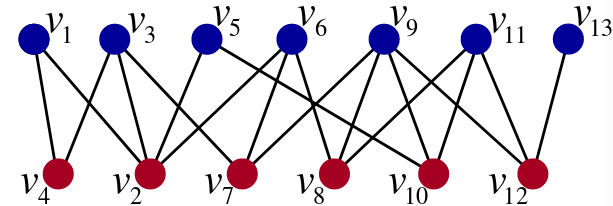
\includegraphics[scale=0.7]{2_colour}
\end{center}
In some cases the last vertex needs a third colour
\begin{center}
	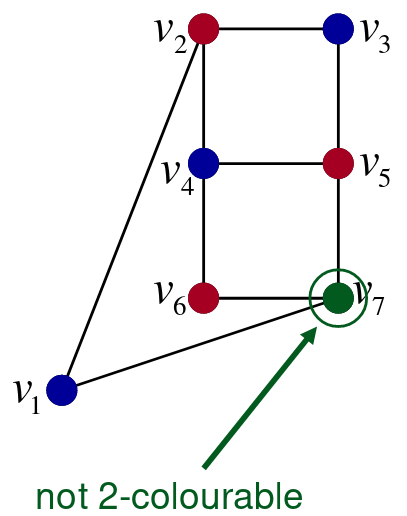
\includegraphics[scale=0.7]{2_colour1}
\end{center}
\section{Bipartite graphs}
\begin{itemize}
	\item Therefore:
	\begin{itemize}
		\item Using the greedy 2 colouring algorithm we can decide whether a given graph is bipartite
	\end{itemize}
	\item Is there any other way to do this?
\end{itemize}
Theorem: A graph is bipartite if, and only if it has no cycles with odd length
\begin{itemize}
	\item Can we use this theorem algorithmically? There can be too many cycles in a graph (exponential)
	\item we can not check all of them efficiently
\end{itemize}
\section{Greedy colouring}
\begin{itemize}
	\item Can the greedy algorithm solve 3 colouring?
\end{itemize}
\begin{center}
	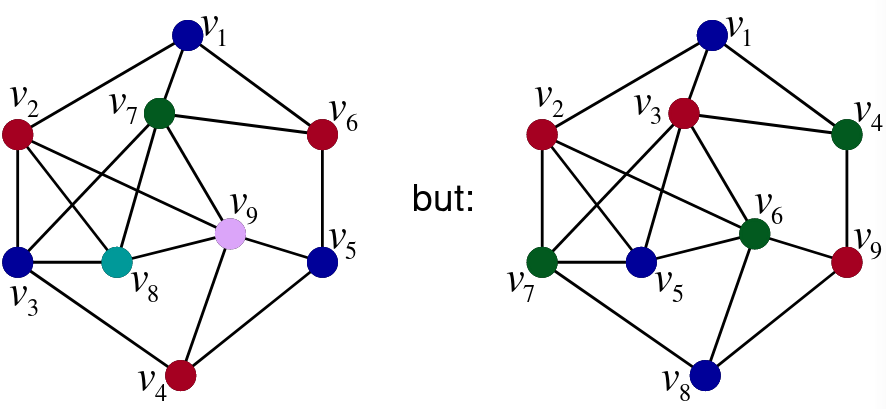
\includegraphics[scale=0.7]{3_colour}
\end{center}
greedy can not be used for 3 colouring
\section{Colouring of planar graphs}
Consider an arbitrary map:
\begin{itemize}
	\item We want to distinguish different countries using different colours
	\item How many colours do we need
\end{itemize}
This is the famous 4 colour problem.\\
How can we model a map by a graph
\begin{itemize}
	\item region of the map $\leftrightarrow$ vertex of the graph
	\item an edge when two regions have common borders
\end{itemize}
Planar graphs:
\begin{itemize}
	\item the graphs that are obtained by maps equivalently
	\item the graphs that can be drawn on the plane such that no two edges cross each other
\end{itemize}
\end{document}